\documentclass[a4paper,8pt]{extarticle}

%%% Работа с русским языком
\usepackage{cmap}					% поиск в PDF
\usepackage{mathtext} 				% русские буквы в формулах
\usepackage[T2A]{fontenc}			% кодировка
\usepackage[utf8]{inputenc}			% кодировка исходного текста
\usepackage[english,russian]{babel}	% локализация и переносы

%%% Дополнительная работа с математикой
\usepackage{amsmath,amsfonts,amssymb,amsthm,mathtools} % AMS
\usepackage{icomma}
\usepackage{physics}
\usepackage{multicol}
\usepackage{bm}
\usepackage{mathrsfs}
\usepackage{verbatim}

%%% Номера формул
%\mathtoolsset{showonlyrefs=true} 
%\usepackage{leqno} 

%%% Свои команды
\DeclareMathOperator{\sgn}{sgn}

\usepackage{csquotes} 
\usepackage[backend=biber,style=authoryear,language=auto]{biblatex}
\addbibresource{source.bib}


%%% Работа с графикой
\usepackage{graphicx}
\graphicspath{{images/}}  
\setlength\fboxsep{3pt} 
\setlength\fboxrule{1pt} 
\usepackage{wrapfig} 
\usepackage{tikz}
\usepackage{pgfplots}
\usepackage{pgfplotstable}
\usepgfplotslibrary{polar}
\pgfplotsset{compat=1.18} 

%%% Работа с таблицами
\usepackage{array,tabularx,tabulary,booktabs}
\usepackage{longtable}  
\usepackage{multirow} 
\usepackage{caption2}[2008/03/29]
\usepackage{soul} 

%%% Теоремы
\theoremstyle{plain} 
\newtheorem{theorem}{Th}[section]
\newtheorem{proposition}[theorem]{Proposition}
 
\theoremstyle{definition} 
\newtheorem{corollary}{Corollary}[theorem]
\newtheorem{problem}{Problem}[section]
\newtheorem{definition}{Def}[section]
 
\theoremstyle{remark} 
\newtheorem*{nonum}{Solution}

%%% Программирование
\usepackage{etoolbox} 

%%% Гиперссылки
\usepackage{hyperref}

\usetikzlibrary{knots}
\usepackage{tcolorbox}

%%% Страница
\usepackage{geometry} 
	\geometry{top=20mm, bottom=20mm, left=15mm, right=20mm}

\usepackage{fancyhdr} 
 	\pagestyle{fancy}
 	\renewcommand{\headrulewidth}{1pt}  
    \rhead{\today}
    \lhead{Новохатний Артем, Цыганкова Екатерина, Мифтахов Эльдар}

\usepackage{setspace} 

\usepackage{lastpage} 

\addbibresource{../source.bib}

\begin{document}
\begin{center}
    \Huge Полиномы Джонса
\end{center}
\begin{multicols}{2}
\subsection*{Глобальная задача:}
Найти инварианты узлов, которые бы позволили различать их между собой. Привести эффективный алгоритм их вычисления.

\columnbreak
\subsection*{Локальная задача:}
Построить инвариантный полином Джонса через скобку Кауфмана, привести алгоритм вычисления, исследовать свойства и вычислить значение на примере простых узлов.
\end{multicols}

\hrule

\begin{multicols}{2}
    \section{Инварианты узлов}
\begin{tcolorbox}
\begin{theorem}\label{thm:Reidemeister}
(Reidemeister 1927) 

Две диаграмы соответствуют изотопным зацеплениям тогда и только тогда, когда их можно получить одну из другой с помощью конечного числа плоских изотопий и преобразований трех типов:
\begin{equation}
\Omega_1:  ~~~~~~ 
  \begin{minipage}{0.06\linewidth}
      \resizebox{\linewidth}{!}{\begin{tikzpicture}
\begin{knot}[
consider self intersections,
clip width=5,
]
\strand[line width=3pt, black]
(-1, -1) to[out=45,in=0,looseness=1]
(0, 1) to[out=180,in=135,looseness=1] (1, -1);
\end{knot}
\end{tikzpicture}}
  \end{minipage} 
  \leftrightarrow
  \begin{minipage}{0.06\linewidth}
      \resizebox{\linewidth}{!}{\begin{tikzpicture}
\begin{knot}[
consider self intersections,
clip width=5,
]
\strand[line width=3pt, black]
(-1, -1) to[out=60,in=180,looseness=1]
(0, 1) to[out=0,in=120,looseness=1] (1, -1);
\end{knot}
\end{tikzpicture}}
  \end{minipage} 
  \leftrightarrow
  \begin{minipage}{0.06\linewidth}
      \resizebox{\linewidth}{!}{\begin{tikzpicture}
\begin{knot}[
consider self intersections,
flip crossing = 1,
clip width=5,
]
\strand[line width=3pt, black]
(-1, -1) to[out=45,in=0,looseness=1]
(0, 1) to[out=180,in=135,looseness=1] (1, -1);
\end{knot}
\end{tikzpicture}}
  \end{minipage} 
\end{equation}

\begin{equation}
\Omega_2:  ~~~~~~ 
  \begin{minipage}{0.06\linewidth}
      \resizebox{\linewidth}{!}{\begin{tikzpicture}
\begin{knot}[
consider self intersections,
clip width=5,
]
\strand[line width=3pt, black]
(-1, -1) to[out=45,in=-90,looseness=1]
(0.5, 0) to[out=90,in=-45,looseness=1] (-1, 1);
\strand[line width=3pt, black]
(1, -1) to[out=135,in=-90,looseness=1]
(-0.5, 0) to[out=90,in=-135,looseness=1] (1, 1);
\end{knot}
\end{tikzpicture}}
  \end{minipage} 
  \leftrightarrow
  \begin{minipage}{0.06\linewidth}
      \resizebox{\linewidth}{!}{\begin{tikzpicture}
\begin{knot}[
consider self intersections,
clip width=5,
]
\strand[line width=3pt, black]
(-1, -1) to[out=60,in=-90,looseness=1]
(-0.5, 0) to[out=90,in=-60,looseness=1] (-1, 1);
\strand[line width=3pt, black]
(1, -1) to[out=120,in=-90,looseness=1]
(0.5, 0) to[out=90,in=-120,looseness=1] (1, 1);
\end{knot}
\end{tikzpicture}}
  \end{minipage} 
\end{equation}

\begin{equation}
\Omega_3:  ~~~~~~ 
  \begin{minipage}{0.06\linewidth}
      \resizebox{\linewidth}{!}{\begin{tikzpicture}
\begin{knot}[
consider self intersections,
clip width=5,
]
\strand[line width=3pt, black]
(-1, 0) to[out=30,in=180,looseness=1] 
(0, 0.5) to[out=0,in=150,looseness=1] (1, 0);
\strand[line width=3pt, black]
(-1, -1) to[out=20,in=-120,looseness=1] (1, 1);
\strand[line width=3pt, black]
(1, -1) to[out=160,in=-60,looseness=1] (-1, 1);
\end{knot}
\end{tikzpicture}}
  \end{minipage} 
  \leftrightarrow
  \begin{minipage}{0.06\linewidth}
      \resizebox{\linewidth}{!}{\begin{tikzpicture}
\begin{knot}[
consider self intersections,
clip width=5,
]
\strand[line width=3pt, black]
(-1, 0) to[out=-30,in=180,looseness=1] 
(0, -0.5) to[out=0,in=-150,looseness=1] (1, 0);
\strand[line width=3pt, black]
(1, 1) to[out=-160,in=60,looseness=1] (-1, -1);
\strand[line width=3pt, black]
(-1, 1) to[out=-20,in=120,looseness=1] (1, -1);
\end{knot}
\end{tikzpicture}}
  \end{minipage} 
\end{equation}

\end{theorem}
\end{tcolorbox}

Теорема \ref{thm:Reidemeister} показывает, что
при построении инвариантов узлов достаточно
проверить, что они сохраняются на преобразованиях 
Рейдемейстера $\Omega_1, \Omega_2, \Omega_3$

\section{Скобка Кауфмана}

\begin{tcolorbox}
\begin{definition}
Аксиомы скобки Кауфмана

\parencite{khovanov}:

    \begin{equation}
    \left\langle 
    \begin{minipage}{0.06\linewidth}
    \resizebox{\linewidth}{!}{\begin{tikzpicture}
\begin{knot}[
consider self intersections,
clip width=5,
]
\strand[line width=3pt, black]
(-1, -1) to[out=45,in=-135,looseness=1] (1, 1);
\strand[line width=3pt, black]
(-1, 1) to[out=-45,in=135,looseness=1] (1, -1);
\end{knot}
\end{tikzpicture}}
    \end{minipage} \right\rangle = 
    \left\langle 
    \begin{minipage}{0.06\linewidth}
    \resizebox{\linewidth}{!}{\begin{tikzpicture}
\begin{knot}[
consider self intersections,
clip width=5,
]
\strand[line width=3pt, black]
(-1, -1) to[out=60,in=-90,looseness=1]
(-0.5, 0) to[out=90,in=-60,looseness=1] (-1, 1);
\strand[line width=3pt, black]
(1, -1) to[out=120,in=-90,looseness=1]
(0.5, 0) to[out=90,in=-120,looseness=1] (1, 1);
\end{knot}
\end{tikzpicture}}
    \end{minipage} \right\rangle - q
    \left\langle 
    \begin{minipage}{0.06\linewidth}
    \resizebox{\linewidth}{!}{\begin{tikzpicture}
\begin{knot}[
consider self intersections,
clip width=5,
]
\strand[line width=3pt, black]
(-1, -1) to[out=30,in=180,looseness=1]
(0, -0.5) to[out=0,in=150,looseness=1] (1, -1);
\strand[line width=3pt, black]
(-1, 1) to[out=-30,in=180,looseness=1]
(0, 0.5) to[out=0,in=-150,looseness=1] (1, 1);
\end{knot}
\end{tikzpicture}}
    \end{minipage} \right\rangle
    \label{eq:skein-kaufman}
    \end{equation}

    \begin{equation}
    \langle L_1 \cup L_2\rangle = \langle L_1\rangle \langle L_2 \rangle
    \end{equation}

    \begin{equation}
    \left\langle 
    \begin{minipage}{0.06\linewidth}
    \resizebox{\linewidth}{!}{\begin{tikzpicture}
\begin{knot}
\strand[line width=3pt, black] 
(0,0) circle[radius=1cm];
\end{knot}
\end{tikzpicture}}
    \end{minipage} \right\rangle = q + q^{-1}
    \end{equation}
\label{def:kauf-brack}
\end{definition}
\end{tcolorbox}

Под отрицательным сглаживанием будем понимать первое разрешение в
\eqref{eq:skein-kaufman}, а положительным - второе\footnote{Важно
 отметить, что если перекресток поменяется на противоположный, то
 и обозначения сглаживаний поменяются местами}. Каждый перекресток
 в узле мы можем сгладить одним из этих двух способов. Сгладив все $n$
 перекрёстков, мы получим диаграмму из некоторого числа $p$ кружочков.
 Всего у нас $2^n$ таких диаграмм, которые мы будем именовать
 состояниями $s$, каждое из которых соответствует разным сглаживаниям
 с $\gamma$ положительных сглаживаний.
 Тогда исходя из \ref{def:kauf-brack} получаем выражение для скобки
 Кауфмана в виде статсуммы:

 \begin{equation}
  \langle L \rangle=\sum_s (-q)^{\gamma} (q + q^{-1})^p
  \label{eq:statsum}
 \end{equation}

 Для разъяснения построения \eqref{eq:statsum} см. Рис.\ref{fig:bar-natan-1}

Заметим, что кружочку можно сопоставить двумерное градуированное
пространство $V$, размерность которого будет $\text{dim} V = q + q^{-1}$.
Тогда \eqref{eq:statsum} перепишется как:

\begin{equation}
  \langle L \rangle=\sum_s (-q)^{\gamma} (\text{dim} V)^p
  \label{eq:statsum-V}
\end{equation}

Это наблюдение будет полезно для дальнейшей работы с полиномами
Хованова.


\section{Полином Джонса как нормализация скобки Кауфмана}


Скобка Кауфмана на ходах Рейдемейстера:

\begin{equation}
  \left\langle 
    \begin{minipage}{0.06\linewidth}
    \vspace{0pt}
    \resizebox{\linewidth}{!}{\begin{tikzpicture}
\begin{knot}[
consider self intersections,
clip width=5,
]
\strand[line width=3pt, black]
(-1, -1) to[out=45,in=0,looseness=1]
(0, 1) to[out=180,in=135,looseness=1] (1, -1);
\end{knot}
\end{tikzpicture}}
    \end{minipage} \right\rangle = -q^{2}
    \left\langle 
    \begin{minipage}{0.06\linewidth}
    \vspace{0pt}
    \resizebox{\linewidth}{!}{\begin{tikzpicture}
\begin{knot}[
consider self intersections,
clip width=5,
]
\strand[line width=3pt, black]
(-1, -1) to[out=60,in=180,looseness=1]
(0, 1) to[out=0,in=120,looseness=1] (1, -1);
\end{knot}
\end{tikzpicture}}
    \end{minipage} \right\rangle \ , \
    \left\langle 
    \begin{minipage}{0.06\linewidth}
    \vspace{0pt}
    \resizebox{\linewidth}{!}{\begin{tikzpicture}
\begin{knot}[
consider self intersections,
flip crossing = 1,
clip width=5,
]
\strand[line width=3pt, black]
(-1, -1) to[out=45,in=0,looseness=1]
(0, 1) to[out=180,in=135,looseness=1] (1, -1);
\end{knot}
\end{tikzpicture}}
    \end{minipage} \right\rangle = q^{-1}
    \left\langle 
    \begin{minipage}{0.06\linewidth}
    \vspace{0pt}
    \resizebox{\linewidth}{!}{\begin{tikzpicture}
\begin{knot}[
consider self intersections,
clip width=5,
]
\strand[line width=3pt, black]
(-1, -1) to[out=60,in=180,looseness=1]
(0, 1) to[out=0,in=120,looseness=1] (1, -1);
\end{knot}
\end{tikzpicture}}
    \end{minipage} \right\rangle
\end{equation}

\begin{equation}
  \left\langle 
    \begin{minipage}{0.06\linewidth}
    \vspace{0pt}
    \resizebox{\linewidth}{!}{\begin{tikzpicture}
\begin{knot}[
consider self intersections,
clip width=5,
]
\strand[line width=3pt, black]
(-1, -1) to[out=45,in=-90,looseness=1]
(0.5, 0) to[out=90,in=-45,looseness=1] (-1, 1);
\strand[line width=3pt, black]
(1, -1) to[out=135,in=-90,looseness=1]
(-0.5, 0) to[out=90,in=-135,looseness=1] (1, 1);
\end{knot}
\end{tikzpicture}}
    \end{minipage} \right\rangle = -q
    \left\langle 
    \begin{minipage}{0.06\linewidth}
    \vspace{0pt}
    \resizebox{\linewidth}{!}{\begin{tikzpicture}
\begin{knot}[
consider self intersections,
clip width=5,
]
\strand[line width=3pt, black]
(-1, -1) to[out=60,in=-90,looseness=1]
(-0.5, 0) to[out=90,in=-60,looseness=1] (-1, 1);
\strand[line width=3pt, black]
(1, -1) to[out=120,in=-90,looseness=1]
(0.5, 0) to[out=90,in=-120,looseness=1] (1, 1);
\end{knot}
\end{tikzpicture}}
    \end{minipage} \right\rangle
\end{equation}

\begin{equation}
  \left\langle 
    \begin{minipage}{0.06\linewidth}
    \vspace{0pt}
    \resizebox{\linewidth}{!}{\begin{tikzpicture}
\begin{knot}[
consider self intersections,
clip width=5,
]
\strand[line width=3pt, black]
(-1, 0) to[out=30,in=180,looseness=1] 
(0, 0.5) to[out=0,in=150,looseness=1] (1, 0);
\strand[line width=3pt, black]
(-1, -1) to[out=20,in=-120,looseness=1] (1, 1);
\strand[line width=3pt, black]
(1, -1) to[out=160,in=-60,looseness=1] (-1, 1);
\end{knot}
\end{tikzpicture}}
    \end{minipage} \right\rangle = 
    \left\langle 
    \begin{minipage}{0.06\linewidth}
    \vspace{0pt}
    \resizebox{\linewidth}{!}{\begin{tikzpicture}
\begin{knot}[
consider self intersections,
clip width=5,
]
\strand[line width=3pt, black]
(-1, 0) to[out=-30,in=180,looseness=1] 
(0, -0.5) to[out=0,in=-150,looseness=1] (1, 0);
\strand[line width=3pt, black]
(1, 1) to[out=-160,in=60,looseness=1] (-1, -1);
\strand[line width=3pt, black]
(-1, 1) to[out=-20,in=120,looseness=1] (1, -1);
\end{knot}
\end{tikzpicture}}
    \end{minipage} \right\rangle
\end{equation}

Попробуем сделать скобку Кауфмана инвариантной. Введём понятия 
положительного и отрицательного пересечения:

\begin{equation}
  +: \ \
  \begin{minipage}{0.06\linewidth}
    \vspace{0pt}
    \resizebox{\linewidth}{!}{\begin{tikzpicture}
\begin{knot}[
consider self intersections,
clip width=5,
]
\strand[line width=3pt, ->, black]
(-1, -1) to[out=45,in=-135,looseness=1] (1, 1);
\strand[line width=3pt, <-, black]
(-1, 1) to[out=-45,in=135,looseness=1] (1, -1);
\end{knot}
\end{tikzpicture}}
    \end{minipage} \ , \ \ -: \ \
    \begin{minipage}{0.06\linewidth}
    \vspace{0pt}
    \resizebox{\linewidth}{!}{\begin{tikzpicture}
\begin{knot}[
consider self intersections,
flip crossing=1,
clip width=5,
]
\strand[line width=3pt, ->, black]
(-1, -1) to[out=45,in=-135,looseness=1] (1, 1);
\strand[line width=3pt, <-, black]
(-1, 1) to[out=-45,in=135,looseness=1] (1, -1);
\end{knot}
\end{tikzpicture}}
    \end{minipage}
\end{equation}

Количесво положительных и отрицательных перекрёстков в узле 
обозначим $n_+$ и $n_-$ соответственно. Попробуем результат скобки
Кауфмана домножить на моном вида $(-1)^{a n_+ + b n_-}q^{c n_+ + d n_-}$,
чтобы добиться инвариантности. Получаем следующий инвариантный 
полином:

\begin{tcolorbox}
\begin{equation}
  \displaystyle
  J(q, L)=(-1)^{n_-}q^{n_+ - 2 n_-}\frac{\langle L \rangle}{\langle
    \begin{minipage}{0.03\linewidth}
    \vspace{0pt}
    \resizebox{\linewidth}{!}{\begin{tikzpicture}
\begin{knot}
\strand[line width=3pt, black] 
(0,0) circle[radius=1cm];
\end{knot}
\end{tikzpicture}}
    \end{minipage}
  \rangle}
  \label{eq:jones}
\end{equation}
\end{tcolorbox}

Под полиномом Джонса будем понимать именно 
\eqref{eq:jones} \footnote{Хотя обычно в литературе
полином Джонса $\tilde{J}$
определяют как $\tilde{J}(t, L) := 
J(-\sqrt{t}, L)$}.


\section{Примеры вычисления и свойства полинома Джонса}

\textbf{Пример 1:} посчитаем зацепления Хопфа разной ориентации:

\begin{equation}
  J\left(
  \begin{minipage}{0.06\linewidth}
    \vspace{0pt}
    \resizebox{\linewidth}{!}{\begin{tikzpicture}
  \begin{knot}[
    clip width=5,
    flip crossing/.list={2}
  ]
    % первая окружность по дугам
    \strand[line width=3pt,->,black] 
      (0,0) arc[start angle=0,end angle=360,radius=1];
    
    % вторая окружность по дугам
    \strand[line width=3pt,->,black] 
      (-1,0) arc[start angle=0,end angle=360,radius=-1];
  \end{knot}
\end{tikzpicture}}
    \end{minipage} \right) = q + q^5
\end{equation}

\begin{equation}
  J\left(
  \begin{minipage}{0.06\linewidth}
    \vspace{0pt}
    \resizebox{\linewidth}{!}{\begin{tikzpicture}
  \begin{knot}[
    clip width=5,
    flip crossing/.list={1}
  ]
    % первая окружность по дугам
    \strand[line width=3pt,->,black] 
      (0,0) arc[start angle=0,end angle=360,radius=1];
    
    % вторая окружность по дугам
    \strand[line width=3pt,<-,black] 
      (-1,0) arc[start angle=0,end angle=360,radius=-1];
  \end{knot}
\end{tikzpicture}}
    \end{minipage} \right) = q^{-1} + q^{-5}
\end{equation}

\textbf{Пример 2:} левый и правый трилистник:

\begin{equation}
  J\left(
  \begin{minipage}{0.06\linewidth}
    \vspace{0pt}
    \resizebox{\linewidth}{!}{\begin{tikzpicture}
\begin{knot}[
consider self intersections,
flip crossing/.list={1, 3}, %переворот пересечений
clip width=5,
]
\strand[line width=3pt, black]
(0, 1) to[out=180,in=-120,looseness=2]
%декартовы координаты
(-30:1) to[out=60,in=120,looseness=2]
%полярные координаты
(210:1) to[out=-60,in=0,looseness=2] (90:1);
\end{knot}
\end{tikzpicture}}
    \end{minipage} \right) = q^{2} + q^{6} - q^{8}
\end{equation}

\begin{equation}
  J\left(
  \begin{minipage}{0.06\linewidth}
    \vspace{0pt}
    \resizebox{\linewidth}{!}{\begin{tikzpicture}
\begin{knot}[
consider self intersections,
flip crossing=2, %переворот пересечений
clip width=5,
]
\strand[line width=3pt, black]
(0, 1) to[out=180,in=-120,looseness=2]
%декартовы координаты
(-30:1) to[out=60,in=120,looseness=2]
%полярные координаты
(210:1) to[out=-60,in=0,looseness=2] (90:1);
\end{knot}
\end{tikzpicture}}
    \end{minipage} \right) = q^{-2} + q^{-6} - q^{-8}
\end{equation}

В ответах прослеживается закономерность относительно степеней $q$.
Этот факт оказывается общим для полинома Джонса:

\begin{tcolorbox}
  \begin{theorem}[О полиноме Джонса зеркального узла]
  \begin{equation}
    J(q, L)=J(q^{-1},\bar{L})\text{, $\bar{L}$ - зеркальный узел}
  \end{equation}
  \label{thm:mirror}
\end{theorem}
\end{tcolorbox}

Доказать \ref{thm:mirror} довольно просто, используя определение
скобки Кауфмана в виде статсуммы.


\section{Определение полинома Джонса через skein-соотношение}
Используя свойство \eqref{eq:skein-kaufman} для противоположных перекрестков, получим:

\begin{equation}
\left\{
\begin{array}{l}
    \left\langle 
    \begin{minipage}{0.06\linewidth}
    \resizebox{\linewidth}{!}{\begin{tikzpicture}
\begin{knot}[
consider self intersections,
clip width=5,
]
\strand[line width=3pt, black]
(-1, -1) to[out=45,in=-135,looseness=1] (1, 1);
\strand[line width=3pt, black]
(-1, 1) to[out=-45,in=135,looseness=1] (1, -1);
\end{knot}
\end{tikzpicture}}
    \end{minipage} \right\rangle = 
    \left\langle 
    \begin{minipage}{0.06\linewidth}
    \resizebox{\linewidth}{!}{\begin{tikzpicture}
\begin{knot}[
consider self intersections,
clip width=5,
]
\strand[line width=3pt, black]
(-1, -1) to[out=60,in=-90,looseness=1]
(-0.5, 0) to[out=90,in=-60,looseness=1] (-1, 1);
\strand[line width=3pt, black]
(1, -1) to[out=120,in=-90,looseness=1]
(0.5, 0) to[out=90,in=-120,looseness=1] (1, 1);
\end{knot}
\end{tikzpicture}}
    \end{minipage} \right\rangle - q
    \left\langle 
    \begin{minipage}{0.06\linewidth}
    \resizebox{\linewidth}{!}{\begin{tikzpicture}
\begin{knot}[
consider self intersections,
clip width=5,
]
\strand[line width=3pt, black]
(-1, -1) to[out=30,in=180,looseness=1]
(0, -0.5) to[out=0,in=150,looseness=1] (1, -1);
\strand[line width=3pt, black]
(-1, 1) to[out=-30,in=180,looseness=1]
(0, 0.5) to[out=0,in=-150,looseness=1] (1, 1);
\end{knot}
\end{tikzpicture}}
    \end{minipage} \right\rangle  ~~ |\cdot q^{-1}\\ \\
    
    \left\langle 
    \begin{minipage}{0.06\linewidth}
    \resizebox{\linewidth}{!}{\begin{tikzpicture}
\begin{knot}[
consider self intersections,
flip crossing = 1,
clip width=5,
]
\strand[line width=3pt, black]
(-1, -1) to[out=45,in=-135,looseness=1] (1, 1);
\strand[line width=3pt, black]
(-1, 1) to[out=-45,in=135,looseness=1] (1, -1);
\end{knot}
\end{tikzpicture}}
    \end{minipage} \right\rangle = 
    \left\langle 
    \begin{minipage}{0.06\linewidth}
    \resizebox{\linewidth}{!}{\begin{tikzpicture}
\begin{knot}[
consider self intersections,
clip width=5,
]
\strand[line width=3pt, black]
(-1, -1) to[out=30,in=180,looseness=1]
(0, -0.5) to[out=0,in=150,looseness=1] (1, -1);
\strand[line width=3pt, black]
(-1, 1) to[out=-30,in=180,looseness=1]
(0, 0.5) to[out=0,in=-150,looseness=1] (1, 1);
\end{knot}
\end{tikzpicture}}
    \end{minipage} \right\rangle - q
    \left\langle 
    \begin{minipage}{0.06\linewidth}
    \resizebox{\linewidth}{!}{\begin{tikzpicture}
\begin{knot}[
consider self intersections,
clip width=5,
]
\strand[line width=3pt, black]
(-1, -1) to[out=60,in=-90,looseness=1]
(-0.5, 0) to[out=90,in=-60,looseness=1] (-1, 1);
\strand[line width=3pt, black]
(1, -1) to[out=120,in=-90,looseness=1]
(0.5, 0) to[out=90,in=-120,looseness=1] (1, 1);
\end{knot}
\end{tikzpicture}}
    \end{minipage} \right\rangle
\end{array}
\right.
\;+\;
\end{equation}

\begin{equation}
  q^{-1} \left\langle 
    \begin{minipage}{0.06\linewidth}
    \resizebox{\linewidth}{!}{\begin{tikzpicture}
\begin{knot}[
consider self intersections,
clip width=5,
]
\strand[line width=3pt, black]
(-1, -1) to[out=45,in=-135,looseness=1] (1, 1);
\strand[line width=3pt, black]
(-1, 1) to[out=-45,in=135,looseness=1] (1, -1);
\end{knot}
\end{tikzpicture}}
    \end{minipage} \right\rangle +
  \left\langle 
    \begin{minipage}{0.06\linewidth}
    \resizebox{\linewidth}{!}{\begin{tikzpicture}
\begin{knot}[
consider self intersections,
flip crossing = 1,
clip width=5,
]
\strand[line width=3pt, black]
(-1, -1) to[out=45,in=-135,looseness=1] (1, 1);
\strand[line width=3pt, black]
(-1, 1) to[out=-45,in=135,looseness=1] (1, -1);
\end{knot}
\end{tikzpicture}}
    \end{minipage} \right\rangle =
    (q^{-1} - q) \left\langle 
    \begin{minipage}{0.06\linewidth}
    \resizebox{\linewidth}{!}{\begin{tikzpicture}
\begin{knot}[
consider self intersections,
clip width=5,
]
\strand[line width=3pt, black]
(-1, -1) to[out=60,in=-90,looseness=1]
(-0.5, 0) to[out=90,in=-60,looseness=1] (-1, 1);
\strand[line width=3pt, black]
(1, -1) to[out=120,in=-90,looseness=1]
(0.5, 0) to[out=90,in=-120,looseness=1] (1, 1);
\end{knot}
\end{tikzpicture}}
    \end{minipage} \right\rangle
    \label{eq:skein-kaufman-cross}
\end{equation}

Аналогично можно наоборот из \eqref{eq:skein-kaufman-cross} 
получить \eqref{eq:skein-kaufman}, 
то есть свойства эквивалентны. 
Но \eqref{eq:skein-kaufman-cross}, 
в отличие от \eqref{eq:skein-kaufman} применимо
для ориентированных узлов и с учетом нормировки
\eqref{eq:jones} дает:

\begin{tcolorbox}
\begin{equation}
q^{-2} J\left (
  \begin{minipage}{0.06\linewidth}
    \resizebox{\linewidth}{!}{\begin{tikzpicture}
\begin{knot}[
consider self intersections,
clip width=5,
]
\strand[line width=3pt, ->, black]
(-1, -1) to[out=45,in=-135,looseness=1] (1, 1);
\strand[line width=3pt, <-, black]
(-1, 1) to[out=-45,in=135,looseness=1] (1, -1);
\end{knot}
\end{tikzpicture}}
    \end{minipage}
\right ) - q^2 J\left (
  \begin{minipage}{0.06\linewidth}
    \resizebox{\linewidth}{!}{\begin{tikzpicture}
\begin{knot}[
consider self intersections,
flip crossing=1,
clip width=5,
]
\strand[line width=3pt, ->, black]
(-1, -1) to[out=45,in=-135,looseness=1] (1, 1);
\strand[line width=3pt, <-, black]
(-1, 1) to[out=-45,in=135,looseness=1] (1, -1);
\end{knot}
\end{tikzpicture}}
    \end{minipage}
\right ) = (q^{-1}-q) J\left (
  \begin{minipage}{0.06\linewidth}
    \resizebox{\linewidth}{!}{\begin{tikzpicture}
\begin{knot}[
consider self intersections,
clip width=5,
]
\strand[line width=3pt, ->, black]
(-1, -1) to[out=60,in=-90,looseness=1]
(-0.5, 0) to[out=90,in=-60,looseness=1] (-1, 1);
\strand[line width=3pt, ->, black]
(1, -1) to[out=120,in=-90,looseness=1]
(0.5, 0) to[out=90,in=-120,looseness=1] (1, 1);
\end{knot}
\end{tikzpicture}}
    \end{minipage}
\right )
\label{eq:skein}
\end{equation}
\end{tcolorbox}

Сотношение \eqref{eq:skein} вместе с требованием $(J(L) = 1 ~~ \forall 
L \sim \begin{minipage}{0.03\linewidth}
    \vspace{0pt}
    \resizebox{\linewidth}{!}{\begin{tikzpicture}
\begin{knot}
\strand[line width=3pt, black] 
(0,0) circle[radius=1cm];
\end{knot}
\end{tikzpicture}}
    \end{minipage})$ однозначно определяют полином
    Джонса. (с.46 \cite{prasolov-sossinsky}).
    Также \eqref{eq:skein} позволяет доказать следующее свойство:
    \begin{tcolorbox}
    \begin{theorem}
      Полином Джонса зацеплений с \textbf{нечетным} числом
      компонент связности содержит только \textbf{четные}
      степени $q$ и наоборот.
    \end{theorem}
    \end{tcolorbox}
\end{multicols}

\begin{figure}[h]
  \centering
  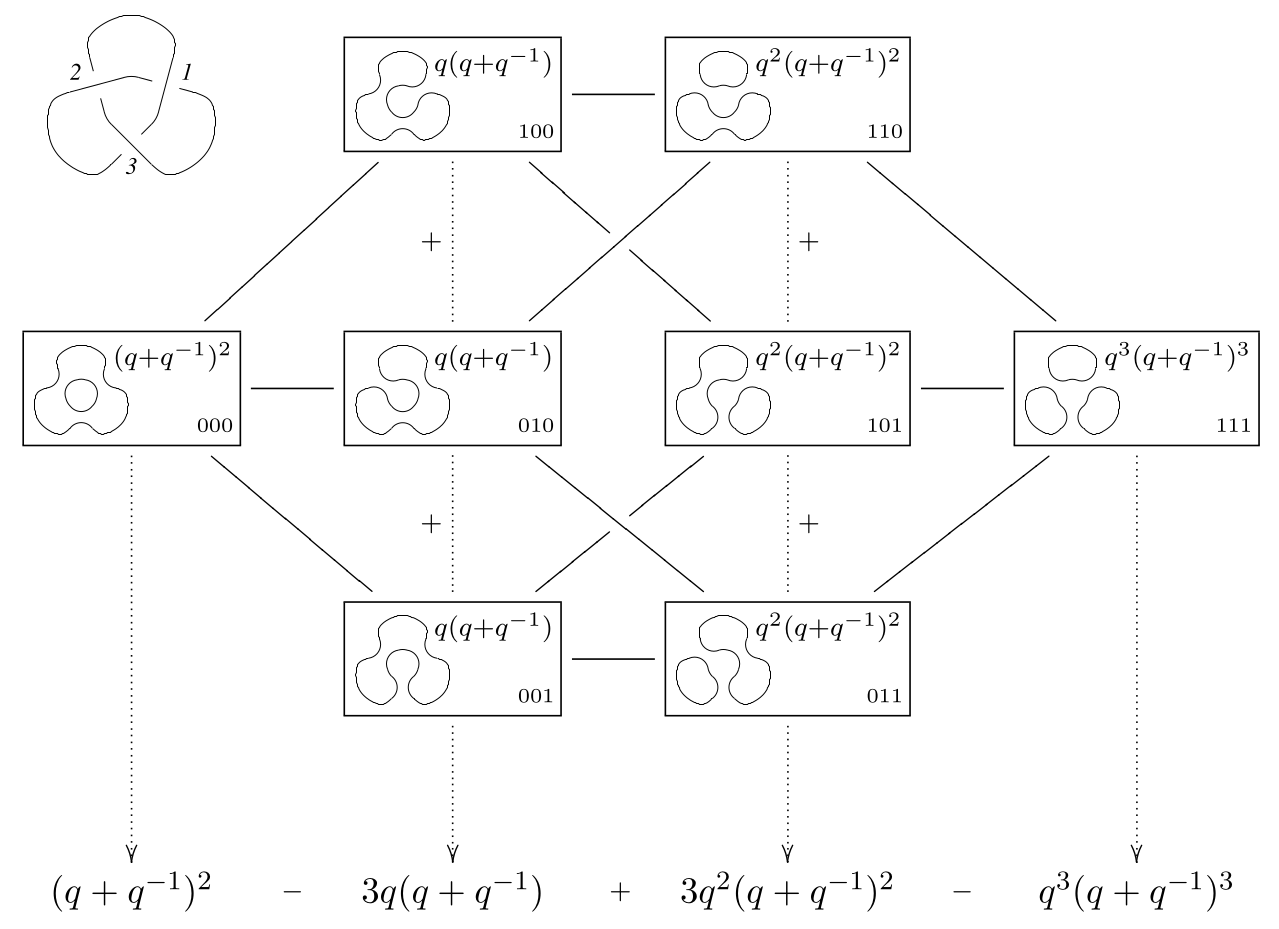
\includegraphics[width=0.8\linewidth]{../img/bar-natan-1.png}
  \caption{Пояснение к скобке Кауфмана, как статсумме \parencite{bar-natan}}
  \label{fig:bar-natan-1}
\end{figure}

\printbibliography
\end{document}

